\documentclass[spanish, fleqn]{article}
\usepackage{babel}
\usepackage{fourier}
\usepackage{amsmath, amsfonts, amsthm, fourier}
\usepackage{float}
\usepackage{graphicx}

\usepackage[colorlinks, urlcolor=blue]{hyperref}

\setlength{\parindent}{0pt}

\title{Ayudantía 2 - Algoritmos y Complejidad\\
Interpolación y Cuadratura}
\author{Exponential Complexers}
\date{}

\begin{document}
\maketitle

\thispagestyle{empty}

\section{Introducción}

Muchas veces olvidamos que los computadores no piensan como nosotros. A pesar de que a nosotros nos gusten las funciones avanzadas y complejas el computador en general prefiere trabajar con casos más generales.\\

Como el computador sabe que cualquier función puede escribirse como una serie polinomial, le gusta aproximar las funciones utilizando polinomios a costa de un pequeño error (el cual existiría de todas maneras debido a la representación de punto flotante).

\section{Interpolación}

A partir de valores exactos de una función desconocida, buscamos el polinomio de menor grado que cumpla con todos esos valores\\

DIBUJO\\

\textbf{Teo:} Existe exactamente un polinomio de grado menor o igual a $n$ que pase por $n+1$ puntos.

\textbf{Dem:} Supongamos $p(x)$ y $q(x)$ polinomios diferentes de grado $\leq n$ que tienen por $n+1$ puntos en común;\\
$\Rightarrow p(x) - q(x)$ es de grado $n$ y tiene $n+1$ ceros,\\
$\Rightarrow p(x) - q(x) = 0$\\

\section{Como Interpolar}

\subsection{Lagrange}

\[ p(x_0) = \sum_{k \leqslant n} f(x_k) \cdot \prod_{\substack{j \leqslant n\\j \neq k}} \frac{x-x_j}{x_k-x_j} \]

\subsection{Newton}

\[Q_0(x) = f(x_0)\]
\[Q_k(x) = \prod_{i \leqslant k - 1} \frac{x-x_i}{x_k - x_i} \cdot \bigg(f(x_k) - Q_{k-1}(x_k)\bigg) + Q_{k-1}(x) \]

\subsubsection{Diferencias divididas}

Para obtener el polinomio interpolador comenzamos dibujando los puntos conocidos $(x_i,y_i)$ en dos columnas verticales.

Luego se construye una pirámide hacia el lado (cada piso tiene 1 celda menos que el piso anterior), en que cada celda contiene la división entre \textbf{la resta de los valores de las dos celdas que la sostienen} y \textbf{los $x_i$ que están en los extremos de la base de la subpirámide que tiene a la celda como cúspide}.

\begin{figure}[H]
\centering
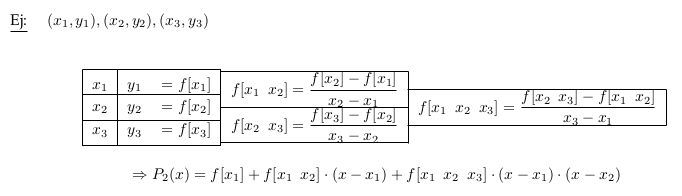
\includegraphics[scale=0.56]{dif_divididas}
\caption{Aplicación del método de las diferencias divididas para 3 puntos.}
\end{figure}

El polinomio interpolador será finalmente, siendo $r_i$ los valores de la primera celda de cada piso $i$.
\begin{align*}
P(x) &= \sum_{i=1}^{n} \left(r_i \cdot \prod_{j=1}^{i-1}(x-x_j)\right)
\end{align*}

\subsection{Sistema de Ecuaciones}

\[\begin{pmatrix}
  1 & x_{0} & x_{0}^{2} & \cdots & x_{0}^{n} \\[0.5em]
  1 & x_{1} & x_{1}^{2} & \cdots & x_{1}^{n} \\[0.5em]
  \vdots  & \vdots  & \ddots & \vdots  \\[0.5em]
  1 & x_{n} & x_{n}^{2} & \cdots & x_{n}^{n}
\end{pmatrix}
\times
\begin{pmatrix}
  a_0 \\[0.5em]
  a-1 \\[0.5em]
  \vdots \\[0.5em]
  a_n
\end{pmatrix}
=
\begin{pmatrix}
  f(x_0) \\[0.5em]
  f(x_1) \\[0.5em]
  \vdots \\[0.5em]
  f(x_n)
\end{pmatrix}
\]

Tiene solución única cuando $\Delta \neq 0$ (Determinante de Vandermonde).\\
Se cumple si $x_i \neq x_j \forall i \neq j$, ya que:
\[\Delta = \prod_{i > j} (x_i - x_j) \]

\subsection{Teorema}
Teniendo $n$ puntos, sólo existe sólo un polinomio interpolador de grado $n-1$ o menor que interpola dichos puntos.
\\\textbf{pregunta} ¿Cuántos existen de grado mayor?

\section{Error de Interpolación}

\textbf{Teo:} sea:\\
$f \in C^{n+1} [a, b]: \mathbb{R} \rightarrow \mathbb{R}$.\\
$Q_n(x)$ polinomio interpolador (grado $n$) en puntos dentro del intervalo.\\

\[\Rightarrow \forall x \in [a, b]\ \exists \zeta \in [a, b] \quad | \quad f(x) - Q_n(x) = \frac{1}{(n+1)!} \cdot f^{(n+1)}(\zeta) \cdot \prod_{0 \leqslant j \leqslant n} (x-x_j) \]

Notar que si $x$ está entre $x_1$ y $x_n$ (suponiendo que los $x_i$ están ordenados) podemos estar seguros de que $x_1 \leq \zeta \leq x_n$, pero $\zeta$ puede llegar incluso a alcanzar $x$ en caso contrario. Esto porque en el intervalo $[a,b]$ deben estar tanto los $x_i$ como $x$.

Otra cosa importante que notar es que el polinomio interpolador de grado $n$ se construye con $n+1$ puntos, por lo tanto, si en algún ejercicio se pide encontrar el error para un polinomio creado a partir de $k$ puntos, no debemos olvidar que debemos reemplazar $n$ por $k-1$ en la fórmula anterior.

\subsection{Puntos de Chebyshev}
Los $n$ puntos que minimizan el máximo valor que puede tomar
\begin{align*}
\left| \prod_{1 \leqslant j \leqslant n} (x-x_j) \right|
\end{align*}
en el intervalo $[-1,1]$ son los puntos:
\begin{align*}
x_i = \cos\left(\frac{(2i-1)\pi}{2n}\right), \qquad i \in \{1..n\}
\end{align*}
Si podemos elegir en qué puntos evaluar la función para crear el polinomio interpolador, conviene elegir estos puntos para minimizar el máximo error de interpolación, si queremos generalizar para un intervalo $[a,b]$ tendremos que:
\begin{align*}
\hat{x}_i = \frac{a+b}{2} + \frac{b-a}{2}x_i
\end{align*}
Y siempre tendremos que:
\begin{align*}
\left| \prod_{1 \leqslant j \leqslant n} (x-x_j) \right| \leq \frac{\left(\frac{b-a}{2}\right)^n}{2^{n-1}}
\end{align*}

\section{Cuadratura}

Se trata de encontrar:
\[ \int_a^b f(x) dx \]
dados ciertos puntos en el intervalo $[a, b]$.

\subsection{Suma de Riemann}

\begin{align*} \int_a^b f(x) dx &\approx \sum_{0 \leqslant j \leqslant n-1} f(x_j) \cdot (x_{j+1} - x_j)\\
&\approx \sum_{0 \leqslant j \leqslant n-1} f\Big(\frac{x_{j+1} + x_j}{2}\Big) \cdot (x_{j+1} - x_j)
\end{align*}

\subsubsection*{Error}
Sea $h = b-a$:
\[e \approx \frac{1}{24} \cdot f''(a) \cdot h^3 \]

\subsection{Cuadratura Gaussiana}
Es mágica, \textbf{PERO}, requiere que uno pueda elegir los $x_i$ que usará para interpolar. La cuadratura Gaussiana generalmente es más barata en términos de tiempo y con $n$ puntos tiene error $0$ para cualquier polinomio de grado $2n-1$.\\

aparte, si queremos calcular la integral de una función en un intervalo $[a, b]$ hay que aplicar una transformación para dejar el cálculo en el intervalo $[-1, 1]$.

\subsubsection*{Ejemplo ($n = 3$)}

Buscamos algo de la forma
\[ \int_{-1}^1 f(x) dx \approx \sum_{i=0}^2 a_i\cdot f(x_i) \]

tomemos $f(x)=x^k$, entonces
\[ \int_{-1}^1 f(x) dx =
\begin{cases}
0 & \text{, } \forall k \text{ impar}\\
\frac{2}{k+1} & \text{, } \forall k \text{ par}
\end{cases}
\]

\textbf{Nos sirve:}
\[ \sum_{i=0}^2 a_i = 2 \]
\[ \sum_{i=0}^2 a_i\cdot x_i^2 = \frac{2}{3} \]
\[ \sum_{i=0}^2 a_i\cdot x_i^4 = \frac{2}{5} \]\\

\textbf{Sospechamos:}
\begin{align*}
        x_0 &= -x_2\\
    x_1 &= 0\\
    a_0 &= a_2
\end{align*}

Despejando las ecuaciones llegamos a que los parámetros para aplicar cuadratura de Gauss con 3 puntos son:
\begin{equation*}
x_0 = -\sqrt{\frac{3}{5}}; \quad x_1 = 0; \quad x_2 = \sqrt{\frac{3}{5}};\\
a_0 = \frac{5}{9}; \quad a_1 = \frac{8}{9}; \quad a_2 = \frac{5}{9}
\end{equation*}

\textbf{Ojo:} Esto nos sirve para integrar en el intervalo $[-1,1]$ ¿Pero qué pasa si queremos integrar el en intervalo $[a,b]$ ?

Tenemos que encontrar los puntos análogos:
\begin{align*}
\hat{x}_i &= \frac{a+b}{2}+\frac{b-a}{2}x_i
\end{align*}

Y cuando tengamos la integral, tenemos que \textbf{multiplicarla} por $\frac{b-a}{2}$ !

\section{Ejercicios}

\begin{enumerate}
\item Encontrar el polinomio interpolador de los puntos $(-1,1),(2,3) y (4,0)$ utilizando diferencias divididas. Suponga que ahora le piden interpolar agregando el punto $(a,b)$. Calcule el nuevo polinomio interpolador reciclando su trabajo anterior.
\item Utilizar interpolación gaussiana con 3 puntos para obtener:
\begin{align*}
\int_{-2}^{3} 2^x dx
\end{align*}
\item Se quiere interpolar, utilizando puntos de Chebyshev, la función $f(x) = e^{2x}$ en el intervalo $[0,r]$, encuentre una cota para el número mínimo de puntos necesarios para que el error sea menor que $\mathfrak{E}$ en dicho intervalo.
\end{enumerate}
\section{Respuestas}
\begin{enumerate}
\item ...
\item ...
\item Tomando la fórmula del error de interpolación:
\begin{align*}
E(x) &= f(x) - Q_n(x) = \frac{1}{(n+1)!} \cdot f^{(n+1)}(\zeta) \cdot \prod_{1 \leq j \leq n} (x-x_j)
\end{align*}
Sabemos que por tratarse de puntos de chebyshev:
\begin{align*}
\left|\prod_{1 \leq j \leq n} (x-x_j)\right| \leq \frac{(r-0)^n}{2^{2n-1}} &= \frac{r^n}{2^{2n-1}}
\end{align*}
Ahora debemos encontrar una cota para:
\begin{align*}
f^{(n+1)}(x) &= 2^{n+1} e^{2x}
\end{align*}
Como esta función es positiva y creciente en el intervalo $[0,r]$, su máximo estará en $x=r$, por lo tanto:
\begin{align*}
|f^{(n)}(x)| \leq |f^{(n)}(r)| = 2^ne^{2r}
\end{align*}
Entonces, el error en dicho intervalo, está acotado por:
\begin{align*}
| E(x) | &=
\left| \frac{1}{n!} \right| \cdot
\left| f^{(n)}(\zeta) \right| \cdot
\left| \prod_{1 \leq j \leq n} (x-x_j) \right|
\\ &\leq \frac{1}{n!} 2^ne^{2r} \frac{r^n}{2^{2n-1}}
\\ &= \frac{e^{2r}}{(n+1)!} \frac{r^n}{2^{n-1}}
\end{align*}
Simplemente hay que elegir un $n$ tal que:
\begin{align*}
\frac{e^{2r}r^n}{n!\cdot 2^{n-1}}\leq \mathfrak{E}
\end{align*}
\end{enumerate}
\end{document}

% LocalWords:  empty Teo Dem subpirámide em dx Gaussiana gaussiana
